%\documentclass[reprint,aps,nofootinbib]{revtex4-1}
\documentclass{report}
\usepackage[margin=1in]{geometry}
\usepackage[utf8]{inputenc}
\usepackage{newtxtext}
\usepackage{amsmath}    % need for subequations
\usepackage{graphicx}   % need for figures
\usepackage{verbatim}   % useful for program listings
\usepackage{color}      % use if color is used in text
\usepackage{subfigure}  % use for side-by-side figures
\usepackage{hyperref}   % use for hypertext links, including those to external documents and URLs
\raggedbottom           % don't add extra vertical space
\usepackage{bbm} % for expectations
\usepackage{cleveref}

\begin{document}

\title{Letter to a Bipaternal Planet}
\author{Aliens}

% tamara: this should probably be the title for the forward, then the main scientific paper would have its own title. Maybe we could format this as a report with three chapters (to start)? 

%\begin{abstract}
%Abstract here.
%\end{abstract}

% tamara: do we need an abstract? seems unnecessary. Instead, we could have the summary of the paper in the forward letter. 

\maketitle
\chapter*{Foreword}
\addcontentsline{toc}{chapter}{Preface}
%\chapter{Foreword}
%!TEX root = main.tex

Greetings, hello, hi, [In voyager, we sent greetings in 55 different languages, which could be cool to merge in one mega greeting/goodbye]

We are individuals from a star system far from yours. 
%, the location of which would be too complicated to describe given your current understanding of the universe. 
We have been assigned by our society the role of surveying the diversity of life forms across our galaxy and have been systematically visiting planets that appear suitable to sustaining life similar to ours. We identified this star system as a possible life-supporting system. As such, we decided to voyage close to this location to assess its viability.
%, planet to planet, for around 30 earth years. Do not worry, we live up to 160 earth years. 
During our latest hyperdrive jump, we nearly collided with a small vessel made by a lifeform unknown to us. Deconstructing this object, we discovered within it a flat golden disk, and upon following the instructions printed on the disk, decoded the information etched into it by your society. 

By studying the stellar diagram on the disk, and cross-referencing this with the ratio of uranium-238 atoms found in the vessel, we realized that your home star system was extremely close to our present location but had been undetected by us because it bears so little in common with our own star system. This fortuitous discovery has allowed us the opportunity to study what kinds of lifeforms can evolve in this seemingly hostile environment. 

The golden disk already contained a great deal of information about you. You appear to understand a subset of mathematical logic and the processes that govern the physical world, which is impressive. There is great diversity in the traits of your life forms, though we did not understand much of what the images depicted. The auditory signals on the disk were intriguing -- some of these signals appear quite sophisticated, such as that labeled ``whale'' and ''Chuck Berry,'' while others are primitive, such as ``Mozart.'' Incidentally, there is, in fact, a 'Turkish'-speaking individual among our crew, who responds to your message with: [Gizem insert something here?]. 

Of all of the information encoded in your disk, however, one feature surprised us most: your apparent reproductive system. Among the images, we found one which depicts two individuals, who look somewhat different from each other and are labeled with symbols (Figure~\ref{fig:1}). The same symbols appeared next to other life forms that different greatly in size and shape (Figure~\ref{fig:2}). These and other images suggest three facts: i) there exist two mating types, ii) one of each mating type is required for reproduction, and iii) the mating types have very different properties. We have, in fact, never observed this in any of the other life forms that we have encountered. Until now we believed that three or more individuals were required for reproduction.

This highly unusual feature of your biology convinced us to study the conditions that may have produced a biparental reproductive system and the consequences of such a system, compared to the more familiar triparental system. We studied your methods of measurement, logic, and communication to gain the ability to transmit our own message to you. Here, we use your units of measurement, your notational system for recording mathematical ideas, and your format for recording knowledge so that you may understand us. Unfortunately, our trajectory only permits a detour of 72 hours, so we are only able to give brief descriptions of our most important findings. 

As we approached your star system, we observed that you use electromagnetic radiation to communicate. We reverse-engineered this communication modality to access your store of knowledge and to relay our own message to you. In this document, we reference knowledge from your own culture that will help you to understand the knowledge that we present to you. We wanted to deposit our message at a location that will ensure that you detect it. One image on your golden disk depicts a structure that appears designed to receive and amplify weak electromagnetic signals (the ``Taj Mahal''). A survey of the surface of your planet revealed an even more optimal signal receiving structure, located near the village of Santa Fe, New Mexico, USA (Figure~\ref{fig:3}). An optical scan of this structure showed it to be inhabited by fourteen of your life forms, and our message has therefore been sent to this location with the hope that these individuals will convey our message to rest of your planet. 

%travels [maybe give exact location of voyager I or II?], we came across a slow moving object. Imagine our surprise when we inspected this object, realizing it was intended as a gift for another form of intelligent life. Included in this object was a flat cylindrical disk encoded with sounds (we were fascinated by these sounds you sent: the sound of the whale is beautiful, the sounds of ``Mozart'' were confusing) as well as several images. 

%Within the cylinder we noticed a few dwellings, one located in the area known as New Mexico, and one called the "Taj Majal" which included several domes. Thus we identified a house in New Mexico with dome-structures like this Taj Majal where we are sending our information. While we imagine there are many topics we could discuss, finding commonalities and differences among our InterPlanetary cultures, one struck us in particular. 

%//[maybe more stuff on the golden record and what we liked about it?]

%The drawings you included in your gold colored disk fascinated and intrigued us. The main picture we determine is a type of 'address', showing us your location, as well as who you, as a species, are. There are several sub-pictures included as well. The picture of one large entity (what you call an "egg"), and multiple small entities from another group (what you call "sperm") may suggest that sexual reproduction among your society is between two individuals (Figure~\ref{fig:1}). The next picture seems to imply that the two entities are associated with two different sexes of humans and these two lead to gestating offspring (Figure~\ref{fig:2}). This image implies that only two individuals are required to reproduce, while the next pictures confirms that reproduction requires only two (different types of) humans. This is surprising: we have never seen a world where only two individuals reproduce. 


\begin{figure}
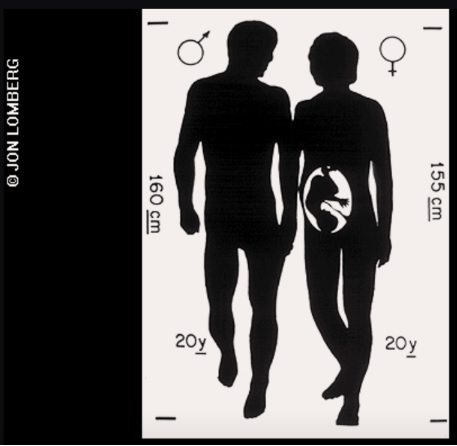
\includegraphics[width=1\columnwidth]{parents_voyager.jpg}
\caption{Two visually distinct life forms, each apparently required for reproduction. Image decoded from the golden disk.
\label{fig:1}}
\end{figure}

\begin{figure}
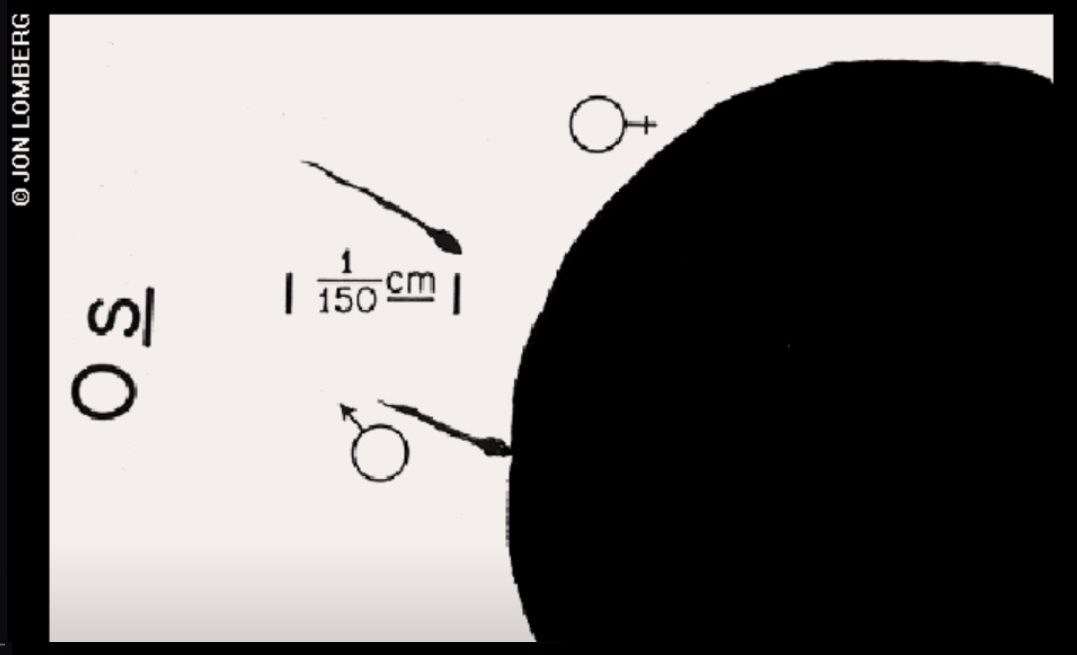
\includegraphics[width=1\columnwidth]{spermandegg_voyager.jpg}
\caption{Entities that are subsets of the life forms depicted in Figure~\ref{fig:1}. These apparently function as the direct mechanisms leading to reproduction and exhibit extremely large size differences. Image decoded from the golden disk.
\label{fig:2}}
\end{figure}

\begin{figure}

\includegraphics[width=1\columnwidth]{rassMandal.jpg}
\caption{Optimal electromagnetic signal receiving structure in Santa Fe, NM.
\label{fig:3}}
\end{figure}


%Again, while we think there are many different points of conversation among our species, the fact that our worlds evolved fundamental differences in reproduction, which then have down-the-line effects for biological family formation, for inequality, species health, and even overarching societal effects (like immigration), we decided to modify our course slightly towards your planet to to understand why you have a two-parent system. Once close enough, we were able to tap into your communication networks and download more information from your planet. We learned many of your languages, watched and read more recordings, and discovered how you humans analyze your own world and its laws, or what you call ``science''. 

%We have 72 hours in your planet's vicinity, and have decided to use this time to send you this report about other planets' reproduction system. In this report, we explored how these systems emerged, how they work biologically, and their societal consequences. We use your scientific writing style and incorporate your own scientific models to make our points more understandable to you.

Several questions still remain regarding your reproductive system. Is this reproductive system limited to ''humans'' or do other organisms also subscribe to two-parent systems? Upon examination of your literature we have determined that most organisms on Earth subscribe to a biparental system, though humans take it to the highest extreme, imbuing societal importance in biparenting. While we have determined that other parental systems among humans exist (for example, what you call polygyny), norms of dominant cultures seem to imbue a superiority to biparenting, even suggesting that single or multi-parenting is deviant and morally inferior. We hope to use the information we send here to suggest that other systems can in fact exist and may in fact imbue certain advantages over biparenting strategies.

In the remainder of this message, we present a series of wide-ranging consequences of the choice of reproductive system, from molecules to societies:

%the following paper we present these ideas scientifically. Below we describe how our system evolved and the implications this has for ecology and society.

\begin{enumerate}
    \item \textbf{The evolution of $n$-parental systems}: In our home star system, which is composed of $N$ planets, all life forms have evolved reproductive systems that require at least three parents. The modal value of parents is 3, though it is possible (and probable) to have more than three parents in our system. Our system is composed of planets that have very limited atmosphere, while your planet has a radiation-protecting ozone. Due to the fact that life on our planets is exposed to, on average, ionizing radiation from 500 to 2,000 Milli-Sievert (mSv), we have higher rates of mutation than life on earth. Due to this, the recombination of genes from multiple parents allows for more viable, and less mutated, life. Recombining genetic material from multiple individuals is highly beneficial in our environment; we are relieved that your planet at least recombines genetic material. Asexual reproduction, we have found, is the worst for offspring and leads to some deleterious mutations out in space!

    \item \textbf{The implications of n parents on ecosystems}: By moving from a 2:1 to a 3:1 parent system, does this reduction in birth rate allow for a slower growth to carrying capacity? What is our population growth in this system?

Having just a replacement rate, you can keep your load on the planetary ecosystem fairly low. So if at a 30 percent marriage rate, and having 3 children, that's replacement rate. This is far below human reproduction rate, which is good.

\item \textbf{The implications of n parents on health}: Three parent systems where parents equally invest in offspring generally lead to greater well-being of children as well as those who gestate the child (what you call the "mother"). In our survey of life on earth we notice that in systems where there are multi-parent systems alongside two-parent system, that multi-parent groups exhibit greater wealth, as well as higher health security for children and mothers.

Despite this, it seems that two-parent systems are the norm. Some seem to suggest it's so that the genetic-material donor (what you call the "father") knows that the offspring is his, while others suggest that the mother drives these two-parent systems, to ensure investment from the father. 

Because of the long-term co-evolution between our high-radiation planet and life, we do not have these same kinds of issues. Equal investment among three parents ensures offspring have low mutation rates, and so each of the N parents are equally invested in their lovely, mutation free, children. 

\item \textbf{Mating selection and Marriage rates}: BLah here.


\item \textbf{How do n-parent systems impact cultural homo/heterogeniety?}: Our interplanetary society evolved to high homogeneity, with mostly one dominant language and culture. However, from the Voyager data as well as other uploaded data from Earth, we notice that your planet has high cultural heterogeneity. A full understanding of this difference between our two civilizations would require more knowledge than is currently possessed about both humanity's deep past are our deep past. However, it this document we present a how-possibly model that points to our system of $n$-partner reproduction, where $n>2$, as a possible explanation for our comparatively high level of cultural homogeneity.

%\textbf{How do n-parent systems impact Health?}: What is the link between std's and mutations? Are mutations lower while STDs higher?

\end{enumerate}

We hope this message will interest you and further your understanding of other possible worlds. 

Peace to all and health forever, 


\chapter{The Biological Evolution of $n$-parental Systems}

\section{Background}

Reproduction is the process by which new organisms are produced by existing organisms. There are a wide variety of reproductive systems that have evolved on Earth and elsewhere, and its evolution depends on its contribution to the fitness of the organism compared to other potential systems. 

Empirically, a reproductive system may consist of several core elements:

\begin{enumerate}

\item \textbf{Sex:} The simplest reproductive system is asexual reproduction. In this case, each individual is capable of independently generating offspring. In the absence of other mechanisms (such as horizontal gene transfer or alternation of generations), each offspring is genetically identical to its parent. Since asexual reproduction does not require any time or energetic cost to finding mates, and all individuals of the population can produce offspring, this strategy can be more efficient and lead to rapid population growth. For example, the asexual reproduction of dandelions (apomixis) on Earth has contributed to its rapid spread. 

Nonetheless, sexual reproduction, where more than one individual is required, is extremely common, both on Earth and elsewhere. This implies that sex can provide strong benefits, since it must overcome the costs of finding mates and coordination among multiple genomes. One important cost of sexual reproduction, first articulated by John Maynard Smith, is the ``two-fold cost of males.'' In cases where sexual reproduction occurs between two sexes, and where only one sex can physically generate offspring, then only half of the population (\emph{i.e.}, only the females) can produce offspring. A mutant that is asexual but otherwise identical to the wildtype organism can on average produce twice as many offspring, since all, rather than half, of its offspring can also produce offspring. Therefore, offspring due to sexual reproduction, where there are two sexes and only one can produce offspring, must, on average, be twice as fit as offspring due to asexual reproduction. 

There are a large number of hypothetical benefits that sexual reproduction can impart on organisms \cite{kondrashov1993classification}. One prominent hypothesis is that sexual reproduction increases the variance of genomes produced in each generation, which can be a bet-hedging strategy in an unpredictable and fluctuating environment. Because sex is so common, it appears that these benefits readily outweigh the ``cost of males'' in many environments. 

\end{enumerate}


\begin{enumerate}
    \item Two-fold cost: ``In an asexual population of stable size, each individual produces an average of one progeny, whereas in a  sexual population with a 1:1 sex ratio each female produces an average of one male and one female progeny. Hence, if a mutation appears causing females to produce two asexual female offspring, its frequency will double in each generation.''~\cite{kondrashov_deleterious_1988}. Also John Maynard SMith, ch. 1, 1978.

    \item Increasing fitness variability /new phenotypes / bringing together good mutations. ``In 1887 Weismann proposed that sex is advantageous because it is 'a source of individual variability furnishing material for  the operation of natural selection. Some data suggest that sexual reproduction can actually cause enhanced fitness of at least a portion of the progeny but the mechanism of this is obscure. Any evolutionary explanation for the maintenance of sexual reproduction can probably fit into Weissmann's framework, because sex does not immediately change allele frequencies and consequently cannot directly improve the popu- lation.''~\cite{kondrashov_deleterious_1988}
    
    \item Mixability~\cite{livnat_mixability_2008}: `` It is commonly believed that, among higher organisms, sexual species (obligate and facultative) are more evolvable than asexual ones (29–31), because they are the founders of wide taxa (12, 29) and are vastly more common (4, 32), while obligate asexuals are mostly recent derivations from sexual ancestors (referred to as ‘’evolutionary dead-ends’’; but see ref. 33) and are phylogenetically sparse (12, 29).”
    
    \item Advantage: removing deleterious mutations. This is the K-model ~\cite{kondrashov_deleterious_1988}.

% From~\cite{power_forces_1976}, ``several plausible models for the evolution of sexuality in multicellular organisms (Williams and Mitton 1973; Williams 1975)''.  But also: ``But multiple mating types would not persist if conditions in each habitat patch were too predictable, for then asexual reproduction would be favored because all asexually produced progeny would be adapted to their habitats while many sexually produced individuals would not.''

\end{enumerate}


\textbf{Number of parents}: For species that reproduce by sexual reproduction, on Earth it is overwhelmingly common for there to be two parents. In other words, genetic material from two individuals combine in order to produce the offspring's genome. While our own life history involves three parents (where the genetic material from three individuals combines to form an offspring, known as triparentalism), this is exceedingly rare on Earth. 

It's not that often discussed or thought about, but sex doesn't have to involve just two parents.  When a zygote is from three parents, it is called \emph{triparentalism}  [OTHER PERRY AND OTHER CITES].  More generally, one can have $n$-parentalism.

Biparentalism almost completely dominates all forms of sexual reproduction on earth.  However, two recent counterexamples have been observed [CITES].  Also, viruses can mix together material from more than two [CITES from Perry].  


Why is non-biparentalism so rare?
\begin{enumerate}
\item Power et al, On Forces of Selection in the Evolution of Mating Types, 1976.~\cite{power_forces_1976} (``formation of an n-ploid zygote by simultaneous or consecutive fusion of three or more gametes''): ``So far as I know, there is no organism requiring the fusion of three or more gametes to form a zygote. There is probably no such organism because of the logistical difficulties of assembling three or more individuals of different sex (or mating type) either simultaneously or consecutively, and individuals requiring two or more mating partners for recombination would thus be at a severe disadvantage in terms of energy expenditure and generation time relative to any others which could successfully reproduce with only a single partner. The n-ploid zygotes might also result in inferior individuals because of mechanical difficulty in segregation of alleles during gametogenesis. An n-ploid individual would probably only be superior if heterosis of n-alleles at a single locus yielded a very great advantage, but even this would probably be offset by the low probability of forming offspring with n-alleles at particular loci. For example, only 2 of the offspring of a union of triploids of genotype ABC would also be ABC, whereas 2 of the offspring of a union between diploids of genotype AB would also be AB, assuming no segregation distortion in either case. Thus the superiority of n-allele heterosis would have to be great enough to more than compensate for reduced proportional output of hybrid offspring, and this would probably require an enormous increase in fecundity.''
\item Perry [CITE] argues that thats there's not necessarily coordination costs.
\item Some have argued that machinery is unclear for it. But not clear that it couldn't be easy with another genetic/biomolecular system.  Perry argues that a 1/4, 1/4, 1/2 system would not be that hard.
\item \cite{hurst_why_1996} briefly discussed multi-parentalism.
\end{enumerate}

Cite Perry. We basically use their model.



%	\item Denis Roze, Disentangling the Benefits of Sex, PLoS Bio, 2012: ``Understanding the evolutionary advantage of sexual reproduction remains one of the most fundamental questions in evolutionary biology. Most of the current hypotheses rely on the fact that sex increases genetic variation, thereby enhancing the efficiency of natural selection; an important body of theoretical work has defined the conditions under which sex can be favoured through this effect. Over the last decade, experimental evolution in model organisms has provided evidence that sex indeed allows faster rates of adaptation. A new study on facultatively sexual rotifers shows that increased rates of sex can be favoured during adaptation to new environmental conditions and explores the cause of this effect. The results provide support for the idea that the benefits of increasing genetic variation may compensate for the short-term costs of sexual reproduction.'' 




\textbf{Mating types:} A subgroup of individuals in a species, which can mate sexually with other subgroups in a systematic pattern.  Review of possible mating type systems, and their combinatorics~\cite{bull_combinatorics_1989}. Emphasizes that vast majority of systems consists of $K$ types, where each type can mate with all other $K-1$ types but not themselves (\emph{self-avoidance}).


%Explain self-avoidance: we have $n$ mating types, who cannot mate with themselves but (usually) all others~\cite{bull_combinatorics_1989}.


If self-avoidance exists, and there is essentially random mixing of mating types, then less common mating types (who can mate with all) will be favored relative to more common mating types,  due to frequency-dependent selection. Absent other effects, this will cause the number of mating types to rise to $n\to \infty$.  This is summarized in a dynamical model by \cite{iwasa_evolution_1987}. This logic is also mentioned earlier, in an informal way, in \cite{power_forces_1976} (`` But if more and more new types were added, each individual would approach universal acceptability and the number of types could come to equal the number of clones.''). Presumably, this will only increase in strength when number of parents to make an offspring increases.

Why do we only observe only two mating types?  Hurst suggests (a somewhat complicated) reason in ~\cite{hurst_why_1996}.  The basic logic (as we understand it) is that it is advantageous to have a single parent contribute the cytoplasm.  With more than two parents, it becomes difficult to guard against selfish mutants, in which two of the parents contribute cytoplasm.  Supports with evidence and citations showing that isogamous systems where mating involves only exchange of nuclear material hundreds or even thousands of mating types can exist.

Power on why not having too many types: ``The maximum number of mating types should be limited by (a) selection against genetically incompatible pairings, (b) competition between members of different mating types, and (c) the between-sexes-choice form of sexual selection operating against genetically incompatible and/or competitively inferior individuals.''~\cite{power_forces_1976}.

Power~\cite{power_forces_1976}: ``In order to understand the selective factors involved in the evolution of mating types, I consider three questions: (1) Why have mating types evolved? (2) Why have more than two types evolved in some populations? (3) What limits the number of types?''



\textbf{Asymmetry}: isogamy vs anisogamy (?). Why do gametes differentiate into one being big (female) and one being small (male)?  This is thought to be the origin of various other sexual dimorphisms.


%Fundamentally, for $n$-parental systems to evolve under natural selection (where $n \geq 3$), it must outcompete other reproductive systems. 



Assume we have $n$ parents and $m$ mating types.  Should we expect to see a symmetry breaking, where the $m$ types are all phenotypically different?


From Power~\cite{power_forces_1976}: ``Parker et al. (1972) have elegantly shown that anisogamy is favored among multicellular organisms if increases in zygote volume produce disproportionately great increases in zygote fitness, but not so much that the benefits of gamete productivity are eliminated. Applying their ideas to protists should yield the same result, i.e., more or less inevitable evolution of anisogamy. What then accounts for the prevalence of isogamy in eucaryotic protists? Probably more constraints are placed on an organism's relative size than a gamete's because it must survive a longer period of time under more variable and less predictable conditions, and thus there may often be but a single optimum size (Parker et al. 1972). Despite the uncommoness of anisogamy among protists, I think it profitable to search for the origin of sexual dimorphism at the protist level because of the possibility anisogamy is primitive with metazoa.''




%!TEX root = main.tex

% Benefit of sex stuff here

\section{An Explanation of Our Triparental System}

Here we review the origin and structure of the $n$-parent system.


\subsection{Why are there $n$ Mating Types?}



From WP, criticisms of \cite{kondrashov_deleterious_1988}: ``There has been much criticism of Kondrashov's theory, since it relies on two key restrictive conditions. The first requires that the rate of deleterious mutation should exceed one per genome per generation in order to provide a substantial advantage for sex. While there is some empirical evidence for it (for example in Drosophila[44] and E. coli[45]), there is also strong evidence against it. Thus, for instance, for the sexual species Saccharomyces cerevisiae (yeast) and Neurospora crassa (fungus), the mutation rate per genome per replication are 0.0027 and 0.0030 respectively. For the nematode worm Caenorhabditis elegans, the mutation rate per effective genome per sexual generation is 0.036.[46] Secondly, there should be strong interactions among loci (synergistic epistasis), a mutation-fitness relation for which there is only limited evidence.[47] Conversely, there is also the same amount of evidence that mutations show no epistasis (purely additive model) or antagonistic interactions (each additional mutation has a disproportionally small effect).'' --- so it works well for high mutation rates and synergistic epistasis --- maybe because their genetic system is system?





%What if took more than 2 parents to make a bebe?


%\chapter{Biological Foundations}


%\section{Why are the Mating Types Asymmetric?}
%%!TEX root = main.tex


Our dominant species has three distinct biological sexes, unlike yours, \emph{homo sapiens}, which has two. As with \emph{home sapiens}, there exists asymmetry and this asymmetry has important consequences for the physical traits of our (and your) species, which in turn has consequences for the organization of our society. Here, we provide a model of gamete asymmetry as an Evolutionarily Stable Strategy (ESS).

% TODO: Determine better names for these species.
Let $m_F$, $m_P$, and $m_C$ be the gamete sizes of our Flower, Pollinator, and Central species. We assume a minimum viable gamete size, $m_0$, and represent the ESS gamete sizes by  $m^*_F$, $m^*_P$, and $m^*_C$. The overall viability, $b$, of the double fertilized ``egg'' is a function of the sum of the gamete sizes, $b=b(m_F,m_P,m_C)$. There are three relevant functions, corresponding to a mutant of each sex attempting to invade the ESS, $W_F(m_F,m_F^*,m_P^*,m_C^*)$, $W_P(m_P,m_F^*,m_P^*,m_C^*)$, and $W_C(m_C,m_F^*,m_P^*,m_C^*)$. While this could be analyzed using the Karush–Kuhn–Tucker (KKT) conditions, the problem is simple enough to intuit the relevant inequalities to enforce where constraints -- notably boundary conditions -- exist.

For simplicity, we assume that each $P$ and $C$ individual follows either a single- or double-mating strategy, and that the probability of each sex adopting a double-mating strategy is, respectively, $q^{(P)}$ and $q^{(C)}$. Given this, each ``mating'' of an $F$ individual faces fertilization competition with probability $p^{(P)} = \frac{2 q^{(P)}}{1+q^{(P)}}$ and each mating of a $P$ individual faces fertilization competition with probability $p^{(C)} = \frac{2 q^{(C)}}{1+q^{(C)}}$. We first consider the ESS condition for $F$ individuals, who adopt a gamete size near the minimum viable size.

Consider now the branching probabilities in Table~\ref{tab:branching} for ``matings''. Whereas increasing gamete size improves the viability of offspring, it reduces the amount of sperm competing in each mating, and we assume that the weighting in this competition is inversely proportional to the gamete size (c.f. Parker). Hence, the fitness of an $F$ mutant following strategy $m_F$ while the others follow $m_P^*$ and $m_C^*$ is

% k1 = 1 - P/2 - C/2 + C*P/6 + C*P^2/12
% k2 = P/2 + C/2 - C*P/6 - C*P^2/12
%\begin{equation}
%  \label{eq:W_F}
%  W(m_F,m_P^*,m_C^*) = b(m_F,m_P^*,m_C^*) %\left[(1-p^{(C)})(1-p^{(P)}) + (1-p^{(C)}) p^{(P)} \frac{1}{\frac{m_F}}{\frac{1}{m_F^*} + \frac{1}{m^*_F} \right]
%\end{equation}
\begin{align}
  \label{eq:W_F}
  W_F(m_F,m_P^*,m_P^*,m_C^*) &= b(m_F,m_P^*,m_C^*)  & \nonumber \\ 
  &\big[& \nonumber \\
  &(1-p^{(C)}) \, (1-p^{(P)})& \nonumber \\
  &+(1-p^{(C)}) \, p^{(P)}& \omega(m_F,m_F^*,1) \nonumber \\
  &+p^{(C)} \, (1-p^{(P)}) \, (1-p^{(P)})& \omega(m_F,m_F^*,1) \nonumber \\
  &+p^{(C)} \, (1-p^{(P)}) \, p^{(P)}& \omega(m_F,m_F^*,2) \nonumber \\
  &+p^{(C)} \, p^{(P)} \, (1-p^{(P)})& \omega(m_F,m_F^*,2) \nonumber \\
  &+p^{(C)} \, p^{(P)} \, p^{(P)} & \omega(m_F,m_F^*,3) \nonumber \\
  &\big]
  %&\frac{1}{m_F} \frac{1}{m_F^*} + \frac{1}{m^*_F} ] 
\end{align}

\noindent where for convenience we define the function $\omega$,
\begin{align*}
\omega(m,m^*,\alpha) = \frac{ \frac{1}{m} }{ \frac{1}{m}+\frac{\alpha}{m^*} }.
\end{align*}

\noindent The first derivative of $\omega$ with respect to $m$ is
\begin{align*}
    \frac{\partial \omega}{\partial m} &= \frac{ -\frac{1}{m^2} }{ \frac{1}{m}+\frac{\alpha}{m^*} }+ \frac{ \frac{1}{m^3} }{ [\frac{1}{m}+\frac{\alpha}{m^*}]^2 }\\
    &=-\frac{1}{m}\omega(m,m^*,\alpha)(1-\omega(m,m^*,\alpha)).
\end{align*}

\noindent Evaluating $\omega$ at $m=m^*$ yields

\begin{align*}
    \omega(m^*,m^*,\alpha) = \frac{1}{1+\alpha}.
\end{align*}
Therefore,
\begin{align*}
  \frac{\partial \omega}{\partial m}|_{m=m^*} &=  -\frac{\alpha}{m^*(1+\alpha)}. 
\end{align*}


%\noindent Let 
%\begin{align*}
%    k_1(p^{(C)}, p^{(P)}) = \frac{p^{(C)} (p^{(P)})^2 }{12} %-\frac{5}{6}p^{(C)}p^{(P)}+\frac{p^{(C)}+p^{(P)}}{2}
%\end{align*}
%and
%\begin{align*}
%    k_2(p^{(C)}, p^{(P)}) = \frac{p^{(C)} (p^{(P)})^2 }{12} %+\frac{1}{6}p^{(C)}p^{(P)}-\frac{p^{(C)}+p^{(P)}}{2}.
%\end{align*}
The first derivative of the $W_F$ with respect to $m_F$ evaluated at $m_F=m_F^*$ is
\begin{align}
    \label{eq:cond_F}
    \frac{\partial W}{\partial m_F}|_{m_F=m_F^*} =
    k_1 \, b'(m^*) - \frac{1}{m_F^*} \, k_2 \, b(m^*)
\end{align}

\noindent where

\begin{equation}
  k_1 = 1 - \frac{p_P + p_C}{2} + \frac{1}{6} p_P p_C + \frac{1}{12} p_P^2 p_C
\end{equation}

\noindent and

\begin{equation}
  k_2 = \frac{p_P + p_C}{2} - \frac{1}{6} p_P p_C - \frac{1}{12} p_P^2 p_C \mbox{.}
\end{equation}

\begin{center}
\begin{tabular}{ |r|r|r|c|c|c| } 
 \hline
             &             && $N_C$ & $N_P$ & $N_F$ \\ 
 $1-p^{(C)}$ & $1-p^{(P)}$ && 1     & 1     & 1 \\ 
 $1-p^{(C)}$ &   $p^{(P)}$ && 1     & 1     & 2 \\ 
   $p^{(C)}$ & $1-p^{(P)}$ & $1-p^{(P)}$ & 1     & 2     & 2 \\ 
   $p^{(C)}$ & $1-p^{(P)}$ & $p^{(P)}$ & 1     & 2     & 3 \\ 
   $p^{(C)}$ & $p^{(P)}$ & $1-p^{(P)}$ & 1     & 2     & 3 \\ 
   $p^{(C)}$ & $p^{(P)}$ & $p^{(P)}$ & 1     & 2     & 4 \\ 
 \hline
\end{tabular}
\label{tab:branching}
\end{center}

\noindent Since $m_F^*=m_0$ at the ESS, the following inequality constraint must be satisfied:
\begin{equation}
  \label{eq:W_F}
    \frac{\partial W_F}{\partial m_F}|_{m_F=m_F^*} < 0 \mbox{.}
\end{equation}
Invoking the so-called Marginal Value Theorem (reference Charnov and Parker here), the optimal investment in offspring viability is achieved when the following condition on overall gamete size is satisfied:

\begin{equation}
  \label{eq:mvt}
  b'(m^*) = \frac{b(m^*)}{m^*} \mbox{.}
\end{equation}

\noindent Combining Equations~\ref{eq:cond_F}, \ref{eq:W_F}, and~\ref{eq:mvt}, the optimal gamete size for $F$ is $m_F^*=m_0$ so long as the following inequality is satisfied:

\begin{equation}
  \label{eq:inequa_F}
  \frac{m_F^*}{m^*} < \frac{k_2}{k_1} = \frac{\frac{p_P + p_C}{2} - \frac{1}{6} p_P p_C - \frac{1}{12} p_P^2 p_C }{ 1 - \frac{p_P + p_C}{2} + \frac{1}{6} p_P p_C + \frac{1}{12} p_P^2 p_C} \mbox{.}
  %\frac{m_F^*}{m^*} < -\frac{k_1}{k_2} = -\frac{ \frac{p^{(C)} (p^{(P)})^2 }{12} -\frac{5}{6}p^{(C)}p^{(P)}+\frac{p^{(C)}+p^{(P)}}{2}}{\frac{p^{(C)} (p^{(P)})^2 }{12} +\frac{1}{6}p^{(C)}p^{(P)}-\frac{p^{(C)}+p^{(P)}}{2}}
\end{equation}


% (1-pC) * (1-pP) N_f



%Although temporally $P$ first retrieves genetic material from one or two F's, then delivers this genetic material to one $C$, it is easier to assess the probabilities in reverse temporal order given the probability 
%of fertilization amounts. The probability of genetic material getting delivered to $C$ with only three individuals represented, which symbolically we shall represent by $\{F:1,P:1,C:1\}$ is $p^{(C)} \. p^{(P)}$. 

%single mating for both $C$

%and competition for each species-specific decision about whether to double- or single-mate. With probability $$
%Given the assumption of only single- or double-mating, the probability of each 

\noindent A similar derivation can be applied to $P$, but with the number $N_P$ standing in for $N_F$ in Table~\ref{tab:branching}. One conclude that

\begin{equation}
  \label{eq:inequa_P}
  \frac{m_P^*}{m^*} < \frac{k_2}{k_1} = \frac{1}{\frac{2}{p_C}-1} \mbox{.}
  %\frac{m_F^*}{m^*} < -\frac{k_1}{k_2} = -\frac{ \frac{p^{(C)} (p^{(P)})^2 }{12} -\frac{5}{6}p^{(C)}p^{(P)}+\frac{p^{(C)}+p^{(P)}}{2}}{\frac{p^{(C)} (p^{(P)})^2 }{12} +\frac{1}{6}p^{(C)}p^{(P)}-\frac{p^{(C)}+p^{(P)}}{2}}
\end{equation}

\subsection{Gamete Asymmetry and its Implications for society}
%!TEX root = main.tex


Our dominant species has three distinct biological sexes, unlike yours, \emph{homo sapiens}, which has two. As with \emph{home sapiens}, there exists asymmetry and this asymmetry has important consequences for the physical traits of our (and your) species, which in turn has consequences for the organization of our society. Here, we provide a model of gamete asymmetry as an Evolutionarily Stable Strategy (ESS).

% TODO: Determine better names for these species.
Let $m_F$, $m_P$, and $m_C$ be the gamete sizes of our Flower, Pollinator, and Central species. We assume a minimum viable gamete size, $m_0$, and represent the ESS gamete sizes by  $m^*_F$, $m^*_P$, and $m^*_C$. The overall viability, $b$, of the double fertilized ``egg'' is a function of the sum of the gamete sizes, $b=b(m_F,m_P,m_C)$. There are three relevant functions, corresponding to a mutant of each sex attempting to invade the ESS, $W_F(m_F,m_F^*,m_P^*,m_C^*)$, $W_P(m_P,m_F^*,m_P^*,m_C^*)$, and $W_C(m_C,m_F^*,m_P^*,m_C^*)$. While this could be analyzed using the Karush–Kuhn–Tucker (KKT) conditions, the problem is simple enough to intuit the relevant inequalities to enforce where constraints -- notably boundary conditions -- exist.

For simplicity, we assume that each $P$ and $C$ individual follows either a single- or double-mating strategy, and that the probability of each sex adopting a double-mating strategy is, respectively, $q^{(P)}$ and $q^{(C)}$. Given this, each ``mating'' of an $F$ individual faces fertilization competition with probability $p^{(P)} = \frac{2 q^{(P)}}{1+q^{(P)}}$ and each mating of a $P$ individual faces fertilization competition with probability $p^{(C)} = \frac{2 q^{(C)}}{1+q^{(C)}}$. We first consider the ESS condition for $F$ individuals, who adopt a gamete size near the minimum viable size.

Consider now the branching probabilities in Table~\ref{tab:branching} for ``matings''. Whereas increasing gamete size improves the viability of offspring, it reduces the amount of sperm competing in each mating, and we assume that the weighting in this competition is inversely proportional to the gamete size (c.f. Parker). Hence, the fitness of an $F$ mutant following strategy $m_F$ while the others follow $m_P^*$ and $m_C^*$ is

% k1 = 1 - P/2 - C/2 + C*P/6 + C*P^2/12
% k2 = P/2 + C/2 - C*P/6 - C*P^2/12
%\begin{equation}
%  \label{eq:W_F}
%  W(m_F,m_P^*,m_C^*) = b(m_F,m_P^*,m_C^*) %\left[(1-p^{(C)})(1-p^{(P)}) + (1-p^{(C)}) p^{(P)} \frac{1}{\frac{m_F}}{\frac{1}{m_F^*} + \frac{1}{m^*_F} \right]
%\end{equation}
\begin{align}
  \label{eq:W_F}
  W_F(m_F,m_P^*,m_P^*,m_C^*) &= b(m_F,m_P^*,m_C^*)  & \nonumber \\ 
  &\big[& \nonumber \\
  &(1-p^{(C)}) \, (1-p^{(P)})& \nonumber \\
  &+(1-p^{(C)}) \, p^{(P)}& \omega(m_F,m_F^*,1) \nonumber \\
  &+p^{(C)} \, (1-p^{(P)}) \, (1-p^{(P)})& \omega(m_F,m_F^*,1) \nonumber \\
  &+p^{(C)} \, (1-p^{(P)}) \, p^{(P)}& \omega(m_F,m_F^*,2) \nonumber \\
  &+p^{(C)} \, p^{(P)} \, (1-p^{(P)})& \omega(m_F,m_F^*,2) \nonumber \\
  &+p^{(C)} \, p^{(P)} \, p^{(P)} & \omega(m_F,m_F^*,3) \nonumber \\
  &\big]
  %&\frac{1}{m_F} \frac{1}{m_F^*} + \frac{1}{m^*_F} ] 
\end{align}

\noindent where for convenience we define the function $\omega$,
\begin{align*}
\omega(m,m^*,\alpha) = \frac{ \frac{1}{m} }{ \frac{1}{m}+\frac{\alpha}{m^*} }.
\end{align*}

\noindent The first derivative of $\omega$ with respect to $m$ is
\begin{align*}
    \frac{\partial \omega}{\partial m} &= \frac{ -\frac{1}{m^2} }{ \frac{1}{m}+\frac{\alpha}{m^*} }+ \frac{ \frac{1}{m^3} }{ [\frac{1}{m}+\frac{\alpha}{m^*}]^2 }\\
    &=-\frac{1}{m}\omega(m,m^*,\alpha)(1-\omega(m,m^*,\alpha)).
\end{align*}

\noindent Evaluating $\omega$ at $m=m^*$ yields

\begin{align*}
    \omega(m^*,m^*,\alpha) = \frac{1}{1+\alpha}.
\end{align*}
Therefore,
\begin{align*}
  \frac{\partial \omega}{\partial m}|_{m=m^*} &=  -\frac{\alpha}{m^*(1+\alpha)}. 
\end{align*}


%\noindent Let 
%\begin{align*}
%    k_1(p^{(C)}, p^{(P)}) = \frac{p^{(C)} (p^{(P)})^2 }{12} %-\frac{5}{6}p^{(C)}p^{(P)}+\frac{p^{(C)}+p^{(P)}}{2}
%\end{align*}
%and
%\begin{align*}
%    k_2(p^{(C)}, p^{(P)}) = \frac{p^{(C)} (p^{(P)})^2 }{12} %+\frac{1}{6}p^{(C)}p^{(P)}-\frac{p^{(C)}+p^{(P)}}{2}.
%\end{align*}
The first derivative of the $W_F$ with respect to $m_F$ evaluated at $m_F=m_F^*$ is
\begin{align}
    \label{eq:cond_F}
    \frac{\partial W}{\partial m_F}|_{m_F=m_F^*} =
    k_1 \, b'(m^*) - \frac{1}{m_F^*} \, k_2 \, b(m^*)
\end{align}

\noindent where

\begin{equation}
  k_1 = 1 - \frac{p_P + p_C}{2} + \frac{1}{6} p_P p_C + \frac{1}{12} p_P^2 p_C
\end{equation}

\noindent and

\begin{equation}
  k_2 = \frac{p_P + p_C}{2} - \frac{1}{6} p_P p_C - \frac{1}{12} p_P^2 p_C \mbox{.}
\end{equation}

\begin{center}
\begin{tabular}{ |r|r|r|c|c|c| } 
 \hline
             &             && $N_C$ & $N_P$ & $N_F$ \\ 
 $1-p^{(C)}$ & $1-p^{(P)}$ && 1     & 1     & 1 \\ 
 $1-p^{(C)}$ &   $p^{(P)}$ && 1     & 1     & 2 \\ 
   $p^{(C)}$ & $1-p^{(P)}$ & $1-p^{(P)}$ & 1     & 2     & 2 \\ 
   $p^{(C)}$ & $1-p^{(P)}$ & $p^{(P)}$ & 1     & 2     & 3 \\ 
   $p^{(C)}$ & $p^{(P)}$ & $1-p^{(P)}$ & 1     & 2     & 3 \\ 
   $p^{(C)}$ & $p^{(P)}$ & $p^{(P)}$ & 1     & 2     & 4 \\ 
 \hline
\end{tabular}
\label{tab:branching}
\end{center}

\noindent Since $m_F^*=m_0$ at the ESS, the following inequality constraint must be satisfied:
\begin{equation}
  \label{eq:W_F}
    \frac{\partial W_F}{\partial m_F}|_{m_F=m_F^*} < 0 \mbox{.}
\end{equation}
Invoking the so-called Marginal Value Theorem (reference Charnov and Parker here), the optimal investment in offspring viability is achieved when the following condition on overall gamete size is satisfied:

\begin{equation}
  \label{eq:mvt}
  b'(m^*) = \frac{b(m^*)}{m^*} \mbox{.}
\end{equation}

\noindent Combining Equations~\ref{eq:cond_F}, \ref{eq:W_F}, and~\ref{eq:mvt}, the optimal gamete size for $F$ is $m_F^*=m_0$ so long as the following inequality is satisfied:

\begin{equation}
  \label{eq:inequa_F}
  \frac{m_F^*}{m^*} < \frac{k_2}{k_1} = \frac{\frac{p_P + p_C}{2} - \frac{1}{6} p_P p_C - \frac{1}{12} p_P^2 p_C }{ 1 - \frac{p_P + p_C}{2} + \frac{1}{6} p_P p_C + \frac{1}{12} p_P^2 p_C} \mbox{.}
  %\frac{m_F^*}{m^*} < -\frac{k_1}{k_2} = -\frac{ \frac{p^{(C)} (p^{(P)})^2 }{12} -\frac{5}{6}p^{(C)}p^{(P)}+\frac{p^{(C)}+p^{(P)}}{2}}{\frac{p^{(C)} (p^{(P)})^2 }{12} +\frac{1}{6}p^{(C)}p^{(P)}-\frac{p^{(C)}+p^{(P)}}{2}}
\end{equation}


% (1-pC) * (1-pP) N_f



%Although temporally $P$ first retrieves genetic material from one or two F's, then delivers this genetic material to one $C$, it is easier to assess the probabilities in reverse temporal order given the probability 
%of fertilization amounts. The probability of genetic material getting delivered to $C$ with only three individuals represented, which symbolically we shall represent by $\{F:1,P:1,C:1\}$ is $p^{(C)} \. p^{(P)}$. 

%single mating for both $C$

%and competition for each species-specific decision about whether to double- or single-mate. With probability $$
%Given the assumption of only single- or double-mating, the probability of each 

\noindent A similar derivation can be applied to $P$, but with the number $N_P$ standing in for $N_F$ in Table~\ref{tab:branching}. One conclude that

\begin{equation}
  \label{eq:inequa_P}
  \frac{m_P^*}{m^*} < \frac{k_2}{k_1} = \frac{1}{\frac{2}{p_C}-1} \mbox{.}
  %\frac{m_F^*}{m^*} < -\frac{k_1}{k_2} = -\frac{ \frac{p^{(C)} (p^{(P)})^2 }{12} -\frac{5}{6}p^{(C)}p^{(P)}+\frac{p^{(C)}+p^{(P)}}{2}}{\frac{p^{(C)} (p^{(P)})^2 }{12} +\frac{1}{6}p^{(C)}p^{(P)}-\frac{p^{(C)}+p^{(P)}}{2}}
\end{equation}

\subsection{Dynamical model for Gamete asymmetry}
\begin{figure}
    \centering
    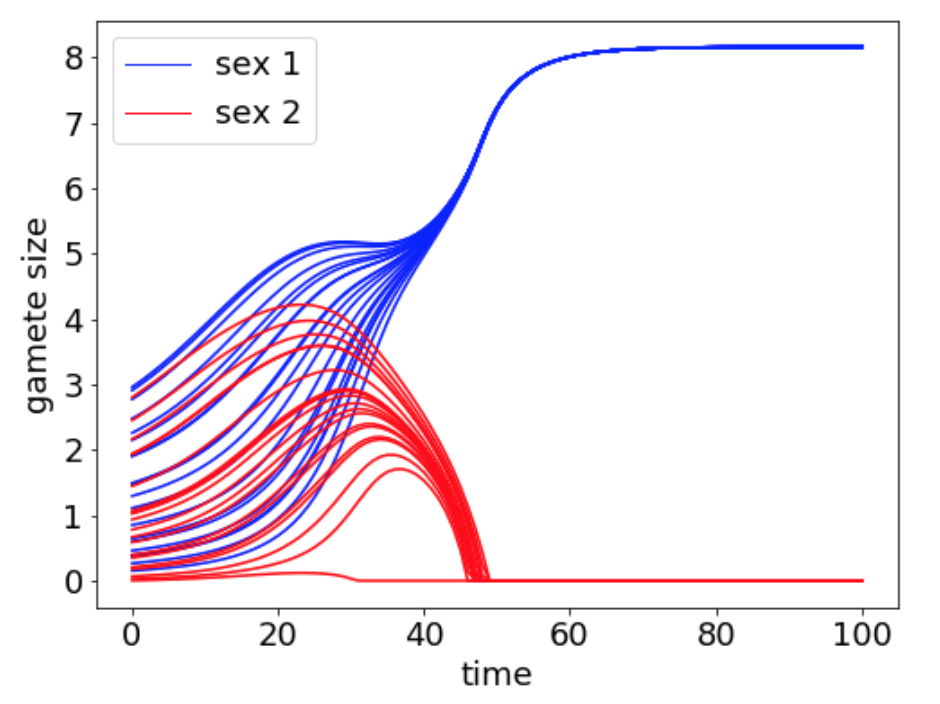
\includegraphics[width = 0.6\textwidth]{vickysFigs/2_sex_run1.png}
    \caption{Simulation for the gamete size evolution in the case of two sexes. One sex evolves to have the minimal size gametes (0, in this model), and the other sex evolves to have large gametes.}
    \label{fig:my_label}
\end{figure}


\subsection{Why unequal birth rates?}
%!TEX root = main.tex

% Benefit of sex stuff here



Human: XX vs XY \\
\scalebox{0.7}{
\begin{tabular}{ |c|c|c| } 
 \hline
  & X & Y \\ 
   \hline
 X & XX & XY \\ 
 X & XX & XY \\ 
 \hline
\end{tabular}
}
\\
2-XX\\
2-XY\\

US: XXX$_f$ vs XXY$_p$ vs XYY$_c$ 

%\begin{tabular}{ |c|c|c|c|c|c|c|c|c|c|c|c| } 
% \hline
% X_c  & X_f & X_f & X_f & Y_c & X_f & X_f & X_f & Y_c & X_f & X_f & X_f \\ 
%  \hline
% X_p & XXX & XXX & XXX & X_p & XXY & XXY & XXY & X_p & XXY & XXY & XXY \\ 
% X_p & XXX & XXX & XXX & X_p & XXY & XXY & XXY & X_p & XXY & XXY & XXY \\ 
% Y_p & XXY & XXY & XXY & Y_p & XYY & XYY & XYY & Y_p & XYY & XYY & XYY \\ 
% \hline
%\end{tabular}
%\\
%6- XXX\\
%6- XYY\\
%15- XXY\\
%1:2.5:1





%XXX$_f$ vs. XX$_p$ vs. X$_c$ \\
%\scalebox{0.7}{
%\begin{tabular}{ |c|c|c|c|c|c|c|c|c|c|c|c| } 
% \hline
% X_c  & X_f & X_f & X_f &  _ & X_f & X_f & X_f & _ & X_f & X_f & X_f \\ 
%  \hline
% X_p & XXX & XXX & XXX & X_p & XX & XX & XX & X_p & XX & XX & XX \\ 
% X_p & XXX & XXX & XXX & X_p & XX & XX & XX & X_p & XX & XX & XX \\ 
% - & XX & XX & XX & _ & X & X & X & _ & X & X & X \\ 
% \hline
%\end{tabular}
%}

%6 - X
%6- X 
%15- XX


braid crossover....



The details of the origin of the biochemistry of our life form, as well as the precise chemistry that forms it, will be discussed in a later section. Here we will focus on explaining our genetics and how it compares to the genetics of your species. For this reason we will talk about our genetic material as sets of double stranded chromosomes so that you are able to understand the analogy. The main distinction however, is that unlike your diploid genomes, where you inherit one copy of each chromosome from one of your two parents, our genome is triploid, where we inherit one copy of each chromosome from one of our three parents. The details of the recombination events occurring pre-gamete formation are discussed in the 'biochemistry textbook' part of the SI and an overview is shown in Figure 

The dynamics of our genetics and how it affects assignment of mating types is surprisingly analogous to yours, but with some key differences which will be expanded upon in the SI. As discussed previously, 
%or after? depending on where we talk about the fact that there are 3 mating types with 2 gamete sizes
our species is composed of three mating types. These mating types are distinguished by three sex-determining genotypes: 'XXY', 'XYY' and 'XYZ'. Each of these mating types produce haploid gametes, and all three gametes need to come together in order to produce a triploid off-spring. Each parent thus contributes a third of its genetic material to the offspring and conversely the offpring's genome is composed of a third of each of its parents genome.
The XYZ mating type produces the largest gamete, that is then fertilized by the other two smaller ones. In your species, you would thus define XYZ as female and the other two as different types of males, although it is important to note that this analogy does not quite match with our genders. The main difference to note is that the two 'male' mating-types each produce only one type of gamete. The XXY genotype only produces X gametes while the XYY genotype only produces Y gametes. It follows that the female, producing all three X, Y and Z gametes, is the one that biologically determines the mating type of the offspring. We have included an extension of a "Punnet square" to illustrate this concept in Table 





\chapter{Social Implications of $n$-parental Systems}
We review a few implications an $n$-parent system would have on greater social structures. We believe there are many consequences beyond this paper, but much of earth's cultural practices and laws are extremely hard for us to understand. Therefore, we concentrated on three different outcomes:\ mating selection, health, and the presence/absence of cultural diversity. We then discuss examples of human societies on Earth whose parenting and child-rearing habits more closely resemble our own. That is, we examine instances of Earthling-human behavior in which more than two parents are directly involved in the raising of children. We find that these societies are characterized by many of the positive features of the $n$-parent families more familiar to us.

\section{Mating Selection}
%!TEX root = main.tex

Monogamy is not the oldest ancestral state; polygyny/polyamory have deep roots in human societies. According to Fortunato (2009; 2015) the evolution of monogamy follows the likelihood of a society wanting to control for resource inheritance. In a monogamous society, paternity can be assured due to high investment by fathers. Low investment can lead to unsure paternity.

In a society, however, where bipartite pairings are not the norm, but tripartite groupings would ensure reproduction, and where these “thrupples” are also monogamous, would the resulting society in fact function differently? Here we examine how a society where three-person-reproduction is the requirement. We assess what impacts this would have on marriage rates, discover how this would influence norms in societies (like passport usage and nationality inheritance) 


In your society as in ours, it is valuable for individuals to form long-term bonds with other potential parents of offspring, in order to take care of the offspring in the long run. 

On Earth, polygyny (male with multiple female spouses) is the default mating system for many mammals, including humans (polygyny is the marriage system of 82\& of societies) \cite{Fortunato2015}.

It seems however that today most marriages on Earth involve two humans, though they can be dissolved. The marriage situation for humans, as well as the evolution of two mating types, lead to labor division and inequalities between the two. 

However, other social systems, such as one wife with multiple husbands, or multiple wives and multiple husbands, do exist. However, it is rare that genetic material from each of these individuals is mixed. One notable exception is among more recent in-vitro fertilization (IVF) couples, where genetic material from two eggs may be combined with that of one sperm. The most common historic combination of more than 2 individuals in a family composes one male and multiple females.



\section{Health}
%!TEX root = main.tex



\section{Emergence of Cultural Homogeneity Under $n$-Parent Reproduction}
%!TEX root = main.tex

\subsubsection{Background to the Problem}

In this section, we provide a simple probabilistic model for calculating an individual's expected number of cultural affinities, such as language or membership in a legal forming group, and show how it provides evidence for an explanatory role for $3$-parent marriage in the emergence of cultural homogeneity in our society.\par 

Suppose that there are $n$ people in the world. Let a possible world $\omega$ be defined as follows:
\begin{equation}
    \omega = \bigcup_{i=1}^{n}(MICA_{i}, M_{i}, CM_{i}, TCA_{i})
\end{equation}
Each $4$-tuple $(MICA_{i}, M_{i}, CM_{i}, TCA_{i})$ represents one individual in the world. Let $WC$ be the set of cultures in the world, which we assume to have infinite but countable cardinality. $MICA_{i}\subseteq WC$ is the cultural affinities that $i$ has independent of marriage. Let $M_{i}$ be the set of other individuals in the population to whom $i$ have ever married. Marriage is a symmetric and transitive (but not reflexive) relation on the set of individuals. $CM_{i}\subseteq WC$ is defined as follows:
\begin{equation}
    CM_{i}=\bigcup_{j\in M_{i}}MICA_{j}\setminus\bigcap_{j\in M_{i}}MICA_{j}
\end{equation}
In other words, $CM_{i}$ is the set of distinct cultures with which $i$'s spouses have marriage-independent affinities. $CM_{i}$ is empty if and only if the individual $i$ is unmarried, so that $M_{i}$ is empty (this assumes no stateless people). Finally, let $TCA_{i}$ be defined as follows:
\begin{equation}
    TCA_{i}=(MICA_{i}\cup CM_{i})\setminus (MICA_{i}\cap CM_{i})
\end{equation}
In other words, $TCA_{i}$ is $i$'s total set of distinct cultural affinities, both independent of marriage and through marriage.\par 

In each possible world $\omega$, assume that $MICA_{i}$ is i.i.d.\ across individuals. Let us define a probability space $(\Omega,\mathcal{P}(\Omega),P(\cdot))$, where $\mathcal{P}(\Omega)$ is the power set of $\Omega$. Let $[TCA_{i}=\alpha]\in\mathcal{P}(\Omega)$ be the set of possible worlds in which the cardinality of $TCA_{i}$ is $\alpha$, i.e.\ the worlds in which $i$ has $\alpha$ distinct cultural affinities. Let $[CM_{i}=\beta]\in\mathcal{P}(\Omega)$ be the set of possible worlds in which the cardinality of $CM_{i}$ is $\beta$, i.e.\ the worlds in which $i$'s spouses have $\beta$ distinct cultural affinities. We can calculate any individual $i$'s expect cultural affinities:
\begin{equation}
    \mathbbm{E}(C_{i})=\sum_{\alpha=1}^{\infty}\alpha P([TCA_{i}=\alpha])
\end{equation}
The law of total probability gives us:
\begin{equation}
    \mathbbm{E}(C_{i}) =  \sum_{\alpha=1}^{\infty}\sum_{\beta=0}^{\infty}\alpha P([TCA_{i}=\alpha]|[CM_{i}=\beta])P([CM_{i}=\beta])
\end{equation}
Which we expand as follows:
\begin{multline}
    \mathbbm{E}(C_{i})= \sum_{\alpha=1}^{\infty}\alpha\big(P([TCA_{i}=\alpha]|[CM_{i}=0])P([CM_{i}=0]) \\ + \  \sum_{\beta=1}^{\infty} P([TCA_{i}=\alpha]|[CM_{i}=\beta])P([CM_{i}=\beta])\big)
\end{multline}
Let $UM_{i}\in\mathcal{P}(\Omega)$ be the set of worlds in which $i$ never marries. By definition, $UM_{i}=[CM_{i}=0]$. So we can re-write the above as follows:
\begin{equation}
    \mathbbm{E}(C_{i})=\sum_{\alpha=1}^{\infty}\alpha\big(P([TCA_{i}=\alpha]|UM_{i})P(UM_{i}) +  \sum_{\beta=1}^{\infty} P([TCA_{i}=\alpha]|[CM_{i}=\beta])P([CM_{i}=\beta])\big)
\end{equation}
Whenever $i$ has never married, their overall cultural affinities match their marriage-independent cultural affinities. This gives us the following:
\begin{equation}
    P([TCA_{i}=\alpha]|UM_{i})=P([MICA_{i}=\alpha])
\end{equation}
So we can re-write the above as follows:
\begin{equation}
    \mathbbm{E}(C_{i})=\sum_{\alpha=1}^{\infty}\alpha\big(P([MICA_{i}=\alpha])P(UM_{i}) + \sum_{\beta=1}^{\infty} P([TCA_{i}=\alpha]|[CM_{i}=\beta])P([CM_{i}=\beta])\big)
\end{equation}
Finally, applying the law of total probability one more time, we get the following:
\begin{multline}
    \mathbbm{E}(C_{i})=\sum_{\alpha=1}^{\infty}\alpha\big(P([MICA_{i}=\alpha])P(UM_{i}) \\ + \    \sum_{\gamma=1}^{\infty}\sum_{\beta=1}^{\infty} P([TCA_{i}=\alpha]|[CM_{i}=\beta]) P([CM_{i}=\beta]|[MICA_{i}=\gamma])P([MICA_{i}=\gamma])\big)
\end{multline}
Based on historical data from our interplanetary system, the prior probability $P([MICA_{i}=\gamma])$, when the mean value of $\gamma$ is $\mu_{\gamma}$, can be found via the following Poisson function:
\begin{equation}
    P([MICA_{i}=\gamma]) \\ = \ f(\gamma,\mu_{\gamma})=\frac{\mu_{\gamma}^{\gamma}e^{-\mu_{\gamma}}}{\gamma!}
\end{equation}
The value of the probability $P([CM_{i}=\beta]|[MICA_{i}=\gamma])$, for any $\beta$ and $\gamma$ is best estimated by the following Poisson function:
\begin{equation}
    P([CM_{i}=\beta]|[MICA_{i}=\gamma])= g(\beta,\gamma)=\frac{(.05+\gamma)^{\beta}e^{-(.05+\gamma)}}{\beta!}
\end{equation}
Thus, the mean number of distinct cultural affinities of a person's marriage partners increases linearly, albeit very slightly, with one's marriage-independent cultural affinities. This reflects the fact that in our society, as on Earth, marriage partners tend to share cultural affinities \cite{Schwartz2013}. The value of the probability $P([TCA_{i}=\alpha]|[CM_{i}=\beta])$ is best estimated by the following Poisson function:
\begin{equation}
    P([TCA_{i}=\alpha]|[CM_{i}=\beta]) = h(\alpha,\beta)=\frac{(.17+\beta^{1.2})^{\alpha}e^{-(.17+\beta^{1.2})}}{\alpha!}
\end{equation}
Thus, the mean number of a person's cultural affinities increases super-linearly with the number of distinct cultural affinities of their marriage partners.\par 

These findings allow us to re-write the equation for $\mathbbm{E}(C_{i})$ as follows:\ 
\begin{equation}
    \mathbbm{E}(C_{i})=\sum_{\alpha=1}^{\infty}\alpha\big(f(\alpha,\mu_{\gamma})P(UM_{i}) + \sum_{\gamma=1}^{\infty}\sum_{\beta=1}^{\infty} h(\alpha,\beta)g(\beta,\gamma)f(\gamma,\mu_{\gamma})\big)
\end{equation}
At this point, we have a framework within which we can state our hypothesis for the generation of homogeneity in our civilization over time. As shown in Section IV.A, the average person under three-partner marriage is much less likely to never marry over the course of their life, and therefore in much more likely to have several partners. More generally, when the number of simultaneous marriage partners is unrestricted, $P(UM_{i})$ is lower than in cases where individuals are permitted only one simultaneous marriage partner. Further, and perhaps more crucially, the following all hold:\ 
\begin{itemize}
\item $f(\gamma,\mu_{\gamma})$ is such that, for any $\gamma$ and $\epsilon$, the probability that $\gamma>\epsilon$ increases as $\mu_{\gamma}$ increases.

\item $g(\beta,\gamma)$ is such that, for any $\beta$ and $\epsilon$, the probability that $\beta>\epsilon$ increases as $\gamma$ increases.

\item $h(\alpha,\beta)$ is such that, for any $\alpha$ and $\epsilon$, the probability that $\alpha>\epsilon$ increases as $\beta$ increases.

\end{itemize}
Thus, $\mathbbm{E}(C_{i})$ is driven up as $\mu_{\gamma}$ increases, i.e.\ as the average number of cultural affinities that a person acquires independently of marriage increases. In a world in which a child can be created via $n$ parents, and inherits the cultural identity of all these parents, and inter-cultural mating is possible, $\mu_{\gamma}$ increases much faster than in a world with the same amount of inter-cultural exchange, but in which a child can only be created by two parents.\par 


\section{Examples of More than Two Parents on Earth}
%!TEX root = main.tex

% Examples polygany 



There is little evidence on earth that polygyny is harmful for individuals. In societies where monogamy and polygyny occur, polygynous groups lead to greater child and woman health and security. Generally speaking, polygynous households are correlated with greater wealth; whether on earth this is due to the fact that wealthier men can have more wives, or those with more wives can aggrandize, is unclear. However, the “polygyny-threshold model” suggests that polygyny will develop when costs associated with sharing a husband can be offset by resource accumulation that would be difficult under monogamy (Lawson et al. 2015, PNAS). What is clear from these studies is that \textit{there is little evidence} that a three-parent group would lead to a decrease in child, mother, or father health. Rather, it seems that evidence points to higher health indices for each individual in this type of family on your own planet.



\chapter{Afterward}
%!TEX root = main.tex

November 4th, 2019

We are sorry to inform you that the transmission ended here. Like you, we were looking forward to more models about these tri-parental world, such as scaling of cities, cost of signaling, or the emergence of monogamous three person marriages. However, we are extremely honored and grateful to have received this much already. 

We hope you enjoyed this inter-space transmission. 

Postdocs of SFI 



\bibliography{ref}{}
\bibliographystyle{plain}

\clearpage



\end{document}
